\documentclass[a4paper,10pt,twoside,openany]{book}

\usepackage[lang=hebrew]{maths}
\usepackage{polynom}
\usepackage{hebrewdoc}
\usepackage{stylish}
\usepackage{lipsum}
\let\bs\blacksquare

\setlength{\parindent}{0pt}

%%%%%%%%%%%%
% Styling %
%%%%%%%%%%%%

\usepackage{enumitem}

%%%%%%%%%%%%%
% Counters  %
%%%%%%%%%%%%%

\setcounter{section}{1}     
            
%BIBLIOGRAPHY
\usepackage[
backend=biber,
style=alphabetic,
]{biblatex}
\addbibresource{bibliography.bib} %Imports bibliography file

\title{
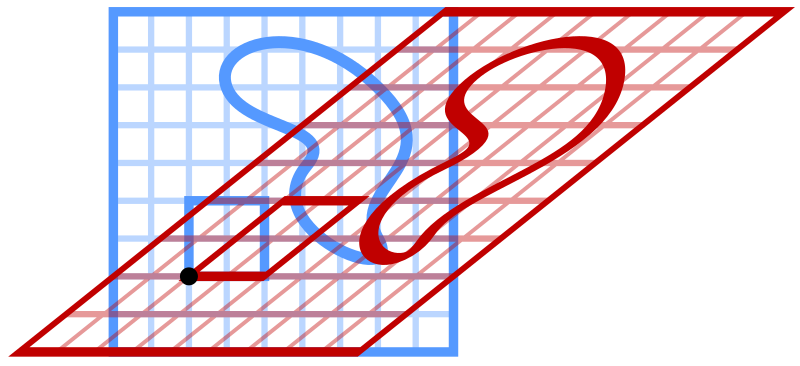
\includegraphics[width=6in]{images/front.png}\\
\vspace{30pt}
\Huge
אלגברה ב' (01040168)
\\
אביב 2025
\\
רשימות תרגולים
\vspace{30pt}
\\
\huge
אלן סורני
\vspace{30pt}
\\
\Large
הרשימות עודכנו לאחרונה בתאריך ה־%
\today
}
\date{}

\begin{document}
\frontmatter
\maketitle
\tableofcontents

\mainmatter

\section*{סימונים}

\begin{itemize}
\item[-]
$\brs{n} = \set{1, \ldots, n}$.
\item[-]
$\sum_{i \in \brs{n}} a_i = \sum_{i=1}^n a_i = a_1 + a_2 + \ldots + a_n$
\item[-] $\Mat_{m \times n}\prs{\mbb{F}}$ הוא מרחב המטריצות עם
$m$
שורות ו־%
$n$
עמודות, עם מקדמים בשדה
$\mbb{F}$.
\item[-]
$\mbb{F}^n = \Mat_{n \times 1}\prs{\mbb{F}}$
\item[-]
$\Mat_{n}\prs{\mbb{F}} = \Mat_{n \times n}\prs{\mbb{F}}$
\item[-]
$\hom_{\mbb{F}}\prs{V,W}$
הוא מרחב ההעתקות הלינאריות
$V \to W$
כאשר
$V,W$
מרחבים וקטוריים מעל
$\mbb{F}$.
\item[-]
$\End_{\mbb{F}}\prs{V} = \hom_{\mbb{F}}\prs{V,V}$
\end{itemize}

\part{חלק ראשון - מרחבים שמורים}

\chapter{חזרה על מטריצות מייצגות}

\section{הגדרות ותכונות בסיסיות}

\begin{definition}[וקטור קואורדינטות]
יהי
$V$
מרחב וקטורי סוף־מימדי מעל שדה
$\mbb{F}$,
יהי
$B = \prs{v_1, \ldots, v_n}$
בסיס של
$V$
ויהי
$v \in V$.
\emph{וקטור הקואורדינטות של
$v$
לפי הבסיס
$B$}
הוא הוקטור
$\brs{v}_B = \pmat{\alpha_1 \\ \vdots \\ \alpha_n}$
כאשר
$\alpha_1, \ldots, \alpha_n \in \mbb{F}$
היחידים עבורם
\[\text{.}v = \sum_{i \in [n]} \alpha_i v_i \coloneqq \alpha_1 v_1 + \ldots + \alpha_n v_n\]
\end{definition}

\begin{remark}
ההעתקה
\begin{align*}
\rho_B \colon V &\to \mbb{F}^n \\
v &\mapsto \brs{v}_B
\end{align*}
היא איזומורפיזם לינארי.
\end{remark}

\begin{definition}[מטריצה מייצגת]
יהיו
$V,W$
מרחבים וקטורים סוף־מימדיים מעל אותו שדה
$\mbb{F}$
עם בסיסים
$B,C$
בהתאמה, ונסמן
\[\text{.} B = \prs{v_1, \ldots, v_n}\]
נסמן גם
$n \coloneqq \dim\prs{V}$
ו־%
$m \coloneqq \dim\prs{W}$.
עבור
$T \in \Hom_{\mbb{F}}\prs{V,W}$
נגדיר
\[\text{.} \brs{T}^B_C = \pmat{\vert & & \vert \\ \brs{T\prs{v_1}}_C & \cdots & \brs{T\prs{v_n}}_C \\ \vert & & \vert} \in \Mat_{m \times n}\prs{\mbb{F}}\]
\end{definition}

\begin{theorem}[כפל מטריצות]
תהי
$A \in \Mat_{m \times n}\prs{\mbb{F}}$
ויהי
$E = \prs{e_1, \ldots, e_m}$
הבסיס הסטנדרטי של
$\mbb{F}^n$.
אז:
\begin{enumerate}[label = (\roman*)]
\item
לכל
$i \in [m]$
מתקיים כי
$A e_i$
העמודה ה־%
$i$
של
$A$.
\item
לכל
$B = \pmat{\vert & & \vert \\ b_1 & \cdots & b_\ell \\ \vert & & \vert} \in \Mat_{n \times \ell}\prs{\mbb{F}}$
מתקיים
$AB = \pmat{\vert & & \vert \\ A b_1 & \cdots & A b_\ell \\ \vert & & \vert}$.
\end{enumerate}
\end{theorem}

\begin{exercisechap}
הראו שניתן לשחזר את ההגדרה של כפל מטריצות משתי התכונות במשפט.
\end{exercisechap}

\begin{remark}
ההעתקה
\begin{align*}
\eta^B_C \colon \Hom_{\mbb{F}}\prs{V,B} &\to \Mat_{m \times n}\prs{\mbb{F}} \\
T &\mapsto \brs{T}^B_C
\end{align*}
היא איזומורפיזם לינארי.
\end{remark}

\begin{proposition}
תהי
$T \in \Hom_{\mbb{F}}\prs{V,W}$
ויהיו
$B = \prs{v_1, \ldots, v_n}$
בסיס של
$V$
ו־%
$C$
בסיס של
$W$.
אז
\[\brs{T}^B_C \brs{v}_B = \brs{T\prs{v}}_C\]
לכל
$v \in V$.
\end{proposition}

\begin{notation}
אם
$B$
בסיס של מרחב וקטורי סוף־מימדי
$V$
ואם
$T \in \End\prs{V}$,
נסמן
$\brs{T}_B \coloneqq \brs{T}^B_B$
ונקרא למטריצה זאת
\emph{המטריצה המייצגת של
$T$
לפי הבסיס
$B$}.
\end{notation}

\begin{notation}
יהי
$V$
מרחב וקטורי סוף־מימדי עם בסיסים
$B,C$.
נסמן
$M^B_C \coloneqq \brs{\id_V}^B_C$.
\end{notation}

\begin{notation}
אם
$A \in \Mat_{n\times n}\prs{\mbb{F}}$,
נסמן
\begin{align*}
T_A \colon \mbb{F}^n &\to \mbb{F}^n \\
\text{.} \hphantom{lalala} v &\mapsto Av
\end{align*}
\end{notation}

\section{תרגילים}

\begin{exercisechap}\label{ex:p(x+1)}
יהי
$V = \mbb{R}_3\brs{x}$
מרחב הפולינום הממשיים ממעלה לכל היותר
$3$,
תהי
\begin{align*}
T \colon \mbb{R}_3\brs{x} &\to \mbb{R}_3\brs{x} \\
p\prs{x} &\mapsto p\prs{x+1}
\end{align*}
ויהי
$B = \prs{1,x,x^2,x^3}$
בסיס של
$V$.
כיתבו את
$\brs{T}_B$.
\end{exercisechap}

\begin{solution}
לפי הגדרת המטריצה המייצגת,
עמודות
$\brs{T}_B$
הן
$\brs{T\prs{x^i}}_B$
עבור
$i \in \set{0,1,2,3}$.
מתקיים
\begin{align*}
T\prs{1} &= 1 \\
T\prs{x} &= x+1 = 1 + x \\
T\prs{x^2} &= \prs{x+1}^2 = 1 + 2x + x^2 \\
T\prs{x^3} &= \prs{x+1}^3 = 1 + 3x + 3x^2 + x^3
\end{align*}
ולכן
\begin{align*}
\brs{T\prs{1}}_B &= e_1 \\
\brs{T\prs{x}}_B &= e_1 + e_2 \\
\brs{T\prs{x^2}}_B &= e_1 + 2 e_2 + e_3 \\
\brs{T\prs{x^3}}_B &= e_1 + 3 e_2 + 3 e_3 + e_4
\end{align*}
ואז
\begin{align*}
\text{.} \brs{T}_B &= \pmat{1 & 1 & 1 & 1 \\ 0 & 1 & 2 & 3 \\ 0 & 0 & 1 & 3 \\ 0 & 0 & 0 & 1}
\end{align*}
\end{solution}

\begin{exercisechap}
יהי
$V = \Mat_{2 \times 2}\prs{\mbb{C}}$,
תהי
\begin{align*}
T \colon V &\to V \\
A &\mapsto \frac{1}{2} \prs{A - A^t}
\end{align*}
ויהי
\[E = \prs{E_{1,1}, E_{1,2}, E_{2,1}, E_{2,2}} \coloneqq \pmat{\pmat{1 & 0 \\ 0 & 0}, \pmat{0 & 1 \\ 0 & 0}, \pmat{0 & 0 \\ 1 & 0}, \pmat{0 & 0 \\ 0 & 1}}\]
\emph{הבסיס הסטנדרטי של
$V$}.
כיתבו את
$\brs{T}_E$.
\end{exercisechap}

\begin{solution}
כמו מקודם, נחשב את
$\brs{T\prs{E_{i,j}}}_E$
כיוון שאלו עמודות
$\brs{T}_E$.
מתקיים
\begin{align*}
T\prs{E_{1,1}} &= \frac{1}{2} \prs{E_{1,1} - E_{1,1}} = 0 \\
T\prs{E_{1,2}} &= \frac{1}{2} \prs{\pmat{0 & 1 \\ 0 & 0} - \pmat{0 & 0 \\ 1 & 0}} = \frac{1}{2} E_{1,2} - \frac{1}{2} E_{2,1} \\
T\prs{E_{2,1}} &= \frac{1}{2} \prs{E_{2,1} - E_{1,2}} = \frac{1}{2} E_{2,1} - \frac{1}{2} E_{1,2} \\
\text{,} T\prs{E_{2,2}} &= \frac{1}{2} \prs{E_{2,2} - E_{2,2}} = 0 \\
\end{align*}
לכן
\begin{align*}
\brs{T\prs{E_{1,1}}}_E &= 0 \\
\brs{T\prs{E_{1,2}}}_E &= \frac{1}{2} e_2 - \frac{1}{2} e_3 \\
\brs{T\prs{E_{2,1}}}_E &= -\frac{1}{2} e_2 + \frac{1}{2} e_3 \\
\brs{T\prs{E_{2,2}}}_E &= 0
\end{align*}
ואז
\begin{align*}
\text{,} \brs{T}_E &= \pmat{0 & 0 & 0 & 0 \\ 0 & \frac{1}{2} & -\frac{1}{2} & 0 \\ 0 & -\frac{1}{2} & \frac{1}{2} & 0 \\ 0 & 0 & 0 & 0}
\end{align*}
כנדרש.
\end{solution}

\begin{exercisechap}
יהי
$V = \Hom_{\mbb{R}}\prs{\mbb{R}^2, \mbb{R}}$
עם הבסיס
$B = \prs{f_1, f_2}$
כאשר
\begin{align*}
f_1\prs{\pmat{x \\ y}} &= x \\
\text{,} f_2\prs{\pmat{x \\ y}} &= y
\end{align*}
ותהי
\begin{align*}
\text{.} A &= \pmat{1 & 2 \\ 3 & 4} \in \Mat_{2 \times 2}\prs{\mbb{R}}
\end{align*}
מיצאו
$T \in \End_{\mbb{R}}\prs{V}$
עבורו
$\brs{T}_B = A$.
\end{exercisechap}

\begin{solution}
עבור
$T \in \End_{\mbb{R}}\prs{V}$
מתקיים
\[\text{.} \brs{T}_B = \pmat{\vert & \vert \\ \brs{T\prs{f_1}}_B & \brs{T\prs{f_2}}_B \\ \vert & \vert}\]
לכן נדרוש
\begin{align*}
\brs{T\prs{f_1}}_B &= \pmat{1 \\ 2} \\
\text{.} \brs{T\prs{f_2}}_B &= \pmat{3 \\ 4}
\end{align*}
אז
\begin{align*}
T\prs{f_1} &= f_1 + 2 f_2 \\
\text{.} T\prs{f_2} &= 3 f_1 + 4 f_2
\end{align*}
לכן, אם
$f \in V$
איבר כללי, נכתוב
\[f\pmat{x\\y} = \alpha x + \beta y = \alpha f_1 \pmat{x \\ y} + \beta f_2\pmat{x \\ y}\]
ונקבל כי
\begin{align*}
\prs{T\prs{f}}\pmat{x\\y} &= \prs{T\prs{\alpha f_1 + \beta f_2}}\pmat{x\\y}
\\&= \alpha T\prs{f_1}\pmat{x\\y} + \beta T\prs{f_2} \pmat{x\\y}
\\&= \alpha \prs{f_1 + 2 f_2}\pmat{x\\y} + \beta \prs{3 f_1 + 4 f_2} \pmat{x\\y}
\\ \text{.} \hphantom{\prs{T\prs{f}}\pmat{x\\y}} &= \alpha \prs{x + 2 y} + \beta \prs{3 x + 4y}
\end{align*}
\end{solution}

\begin{exercisechap}
תהיינה
$A,B \in \Mat_{m \times n}\prs{\mbb{F}}$
ונניח כי לכל
$v \in \mbb{F}^n$
מתקיים
$Av = Bv$.
אז
$A = B$.
\end{exercisechap}

\begin{solution}
מהנתון, מתקיים
$\prs{A - B}v = 0$
לכל
$v \in \mbb{F}^n$.
בפרט העמודה ה־%
$i$
של
$A-B$,
שהינה
$\prs{A - B}e_i$,
שווה ל־%
$0$.
לכן
$A - B = 0$.
\end{solution}

\begin{proposition}
יהיו
$U,V,W$
מרחבים וקטוריים סוף־מימדיים מעל אותו שדה
$\mbb{F}$
עם בסיסים
$B,C,D$
בהתאמה,
ותהיינה
\begin{align*}
S \in \Hom_{\mbb{F}}\prs{U,V} \\
\text{.} T \in \Hom_{\mbb{F}}\prs{V,W}
\end{align*}
אז
\[\text{.} \brs{T \circ S}^B_D = \brs{T}^C_D \brs{S}^B_C\]
\end{proposition}

\begin{exercisechap} \label{exercisechap:change-of-basis-through-isomorphism}
יהיו
$V,W$
מרחבים וקטוריים סוף־מימדיים מעל שדה
$\mbb{F}$
ותהי
$T \in \Hom_{\mbb{F}}\prs{V,W}$
חד־חד ערכית.

יהיו
\begin{align*}
B &= \prs{v_1, \ldots, v_n} \\
C &= \prs{u_1, \ldots, u_n}
\end{align*}
בסיסים של
$V$
ויהיו
\begin{align*}
B' &= \prs{T\prs{v_1}, \ldots, T\prs{v_n}} \\
\text{.} C' &= \prs{T\prs{u_1}, \ldots, T\prs{u_n}}
\end{align*}
אז
$B',C'$
בסיסים של
$\im\prs{T} = \set{T\prs{v}}{v \in V}$
וגם
$M^B_C = M^{B'}_{C'}$.
\end{exercisechap}

\begin{solution}
כיוון ש־%
$T$
חד־חד ערכית ועל התמונה, צמצום הטווח נותן איזומורפיזם
$T \colon V \riso \im\prs{T}$.
איזומורפיזם שולח בסיס לבסיס, לכן
$B',C'$
בסיסים.

כעת, לכל
$i \in [n]$
נכתוב
\begin{align*}
v_i &= \sum_{j \in \brs{n}} \alpha_{i,j} u_i
\end{align*}
ואז
\begin{align*}
\text{.} M^B_C e_i = \brs{v_i}_C = \pmat{\alpha_{i,1} \\ \vdots \\ \alpha_{i,n}}
\end{align*}
כמו כן,
\begin{align*}
T\prs{v_i}
&=
T\prs{\sum_{i \in [n]} \alpha_{i,j} u_j}
\\&=
\sum_{i \in [n]} \alpha_{i,j} T\prs{u_j}
\end{align*}
ולכן גם
\[\text{.} M^{B'}_{C'} e_i = \brs{T\prs{v_i}}_{C'} = \pmat{\alpha_{i,1} \\ \vdots \\ \alpha_{i,n}}\]
קיבלנו כי כל עמודות המטריצות שוות, ולכן יש שוויון.
\end{solution}

\begin{exercisechap}
תהי
$A \in \Mat_{n \times n}\prs{\mbb{F}}$
הפיכה.
\begin{enumerate}
\item יהי
$E$
הבסיס הסטנדרטי של
$\mbb{F}^n$.
מיצאו בסיס
$B$
של
$\mbb{F}^n$
עבורו
$A = M^B_E$.

\item
מיצאו בסיס
$C$
של
$\mbb{F}^n$
עבורו
$A = M^E_C$.

\item \emph{
(לא הספקנו בתרגול)
}
יהי
$B$
בסיס של
$\mbb{F}^n$.
מיצאו בסיס
$C$
של
$\mbb{F}^n$
עבורו
$A = M^B_C$.

\item \emph{
(לא הספקנו בתרגול)
}
יהי
$V$
מרחב וקטורי ממימד
$n \in \mbb{N}_+$
מעל
$\mbb{F}$,
יהי
$T \in \End_{\mbb{F}}\prs{V}$
איזומורפיזם
ויהי
$B = \prs{v_1, \ldots, v_n}$
בסיס של
$V$.
מיצאו בסיס
$C$
של
$V$
עבורו
$\brs{T}^B_C = A$.
\end{enumerate}
\end{exercisechap}

\begin{solution}
\begin{enumerate}
\item
אם
$B = \prs{v_1, \ldots, v_n}$,
מתקיים מההגדרה כי
\[\text{.} M^B_E = \pmat{\vert & & \vert \\ \brs{v_1}_E & \cdots & \brs{v_n}_E \\ \vert & & \vert} = \pmat{\vert & & \vert \\ v_1 & \cdots & v_n \\ \vert & & \vert}\]
לכן ניקח את
$\prs{v_1, \ldots, v_n}$
להיות עמודות
$A$,
לפי הסדר.

\item
לכל
$v \in \mbb{F}^n$
מתקיים
\[M^C_E M^E_C v = M^C_E \brs{v}_C = \brs{v}_E = v\]
ולכן
$M^E_C = \prs{M^C_E}^{-1}$.
אם ניקח
$C = \prs{u_1, \ldots, u_n}$
כאשר
$u_i$
העמודה ה־%
$i$
של
$A^{-1}$
נקבל מהסעיף הקודם כי
$M^C_E = A^{-1}$
ולכן
$M^E_C = \prs{A^{-1}}^{-1} = A$.
כלומר ניקח,
$u_i = A^{-1} e_i$.

\item
מתקיים
$M^B_C = M^E_C M^B_E$
לכן נרצה שיתקיים
$M^E_C M^B_E = A$
או במילים אחרות
$M^E_C = A \prs{M^B_E}^{-1} = A M^E_B$.
מהסעיף הקודם, נרצה
$C = \prs{u_1, \ldots, u_n}$
כאשר
$u_i$
העמודה ה־%
$i$
של
$\prs{A M^E_B}^{-1} = M^B_E A^{-1}$,
כלומר
\[\text{.} u_i = M^B_E A^{-1} e_i\]

\item
עבור כל בסיס
$C'$
מתקיים
$\brs{T}^B_{C'} = M^B_{C'} \brs{T}^B_B$
לכן נרצה
$M^B_C \brs{T}^B_B = A$.
כיוון ש־%
$T$
איזומורפיזם, המטריצה
$\brs{T}^B_B$
הפיכה, ולכן נרצה
$M^B_C = A \prs{\brs{T}^B_B}^{-1}$.
כעת, אם
$C = \prs{v_1, \ldots, v_n}$
נקבל לפי
\ref{proposition:change-of-basis-through-isomorphism}
עבור האיזומורפיזם
$\rho_B$
כי
$M^B_C = M^E_{\hat{C}}$
כאשר
$\hat{C} = \prs{\brs{v_1}_B, \ldots, \brs{v_n}_B}$.
לכן נחפש
$\hat{C}$
עבורו
$M^E_{\hat{C}} = A \brs{T}_B^{-1}$.
לפי הסעיף השני, נרצה
$\hat{C} = \prs{u_1, \ldots, u_n}$
עבור
\[\text{.} u_i = \prs{A \brs{T}_B^{-1}}^{-1} e_i = \brs{T}_B A^{-1} e_i\]
לכן
\[\text{.} v_i = \rho_B^{-1} \prs{\brs{T}_B A^{-1} e_i}\]
\end{enumerate}
\end{solution}

\begin{exercisechap}[לא הספקנו בתרגול]
יהי
$V = \mbb{C}_3\brs{x}$,
תהי
\begin{align*}
T \colon V &\to V \\
\text{,} \hphantom{lalala} p\prs{x} &\mapsto p\prs{x+1}
\end{align*}
יהי
$E = \pmat{1,x,x^2,x^3}$,
\emph{הבסיס הסטנדרטי}
ותהי
$A = \pmat{0 & 1 & 0 & 0 \\ 1 & 0 & 0 & 0 \\ 0 & 0 & 0 & 1 \\ 0 & 0 & 1 & 0}$.
כיתבו מפורשות בסיס
$C$
של
$V$
עבורו
$A = \brs{T}^E_C$.
\end{exercisechap}

\begin{solution}
לפי התרגיל הקודם, נרצה קודם
$\hat{C} = \prs{u_1, \ldots, u_4}$
כאשר
$u_i = \brs{T}_E A^{-1} e_i$.
חישבנו ב־%
\ref{ex:p(x+1)}
כי
\[\brs{T}_E = \pmat{1 & 1 & 1 & 1 \\ 0 & 1 & 2 & 3 \\ 0 & 0 & 1 & 3 \\ 0 & 0 & 0 & 1}\]
וניתן לראות כי
$A^2 = I$
כלומר
$A^{-1} = A$.
נשים לב כי
\begin{align*}
A e_1 &= e_2 \\
A e_2 &= e_1 \\
A e_3 &= e_4 \\
A e_4 &= e_3
\end{align*}
ואז נקבל
\begin{align*}
u_1 &= \brs{T}_E A^{-1} e_1 = \brs{T}_E e_2 = \pmat{1 \\ 1 \\ 0 \\ 0} \\
u_2 &= \brs{T}_E A^{-1} e_2 = \brs{T}_E e_1 = \pmat{1 \\ 0 \\ 0 \\ 0} \\
u_3 &= \brs{T}_E A^{-1} e_3 = \brs{T}_E e_4 = \pmat{1 \\ 3 \\ 3 \\ 1} \\
\text{,} u_4 &= \brs{T}_E A^{-1} e_4 = \brs{T}_E e_3 = \pmat{1 \\ 2 \\ 1 \\ 0}
\end{align*}
כלומר
\[\text{,} \hat{C} = \prs{\pmat{1 \\ 1 \\ 0 \\ 0}, \pmat{1 \\ 0 \\ 0 \\ 0}, \pmat{1 \\ 3 \\ 3 \\ 1}, \pmat{1 \\ 2 \\ 1 \\ 0}}\]
ולבסוף
\[\text{.} C = \prs{v_1, v_2, v_3, v_4} \coloneqq \prs{1+x, 1, 1+3x+3x^2+x^3, 1+2x+x^2}\]

ליתר ביטחון, נבדוק שהמטריצה המייצגת היא אכן
$A$.
מתקיים
\begin{align*}
T\prs{1} &= 1 = v_2 \\
T\prs{x} &= x+1 = v_1 \\
T\prs{x^2} &= \prs{x+1}^2 = 1+2x+x^2 = v_4 \\
T\prs{x^3} &= \prs{x+1}^3 = 1+3x+3x^2+x^3 = v_3
\end{align*}
ולכן
\begin{align*}
\brs{T}^E_C &= \pmat{\vert & \vert & \vert & \vert \\ \brs{T\prs{1}}_C & \brs{T\prs{x}}_C & \brs{T\prs{x^2}}_C & \brs{T\prs{x^3}}_C \\ \vert & \vert & \vert & \vert}
\\&= \pmat{\vert & \vert & \vert & \vert \\ \brs{v_2}_C & \brs{v_1}_C & \brs{v_4}_C & \brs{v_3}_C \\ \vert & \vert & \vert & \vert}
\\&= \pmat{\vert & \vert & \vert & \vert \\ e_2 & e_1 & e_4 & e_3 \\ \vert & \vert & \vert & \vert}
\\&= A
\end{align*}
כנדרש.
\end{solution}

\chapter{הדטרמיננטה}

\section{הגדרות ותכונות בסיסיות}

\begin{definition}[דטרמיננטה]
תהי
$A \in \Mat_{n \times n}\prs{\mbb{F}}$
מטריצה עם מקדמים בשדה
$\mbb{F}$.
נגדיר את
\emph{הדטרמיננטה}
$\det\prs{A}$
של
$A$
באופן הרקורסיבי הבא.

תהי
$A_{\prs{i,j}}$
המטריצה המתקבלת מ־%
$A$
על ידי הסרת השורה ה־%
$i$
והעמודה ה־%
$j$.
המספר
$\det\prs{A_{\prs{i,j}}}$
נקרא
\emph{המינור}
ה־$\prs{i,j}$ של
$A$
והדטרמיננטה של
$A$
שווה
\begin{align*}
\det\prs{A} &= \sum_{i \in \brs{n}} \prs{-1}^{i+j} a_{i,j} \det\prs{A_{\prs{i,j}}}
\end{align*}
עבור כל
$j \in \brs{n}$
קבוע, ושווה
\begin{align*}
\det\prs{A} &= \sum_{j \in \brs{n}} \prs{-1}^{i+j} a_{i,j} \det\prs{A_{\prs{i,j}}}
\end{align*}
עבור כל
$i \in \brs{n}$
קבוע.
\end{definition}

\begin{theorem}
תהיינה
$A, B, C \in \Mat_{n \times n}\prs{\mbb{F}}$
ונניח כי
$C$
הפיכה.
מתקיימות התכונות הבאות.
\begin{enumerate}
\item $\det\prs{AB} = \det\prs{A} \cdot \det\prs{B}$
\item $\det\prs{C^{-1}} = \prs{\det\prs{C}}^{-1}$
\end{enumerate}
\end{theorem}

\begin{theorem}
\begin{enumerate}
\item החלפת שתי שורות או עמודות במטריצה כופלת את הדטרמיננטה ב־%
$\prs{-1}$.
\item כפל שורה או עמודה במטריצה בסקלר
$\alpha$
כופל את הדטרמיננטה ב־%
$\alpha$.
\item הוספת כפולה שורה או עמודה לשורה או עמודה במטריצה אינה משנה את הדטרמיננטה.
\end{enumerate}
\end{theorem}

\section{תרגילים}

\begin{exercisechap}
חשבו את הדטרמיננטות של המטריצות הבאות.

\begin{enumerate}
\item \[\pmat{1 & 2 & 3 \\ 4 & 5 & 6 \\ 7 & 8 & 9} \in \Mat_{3}\prs{\mbb{R}}\]
\item \[\pmat{0 & 0 & 0 & 1 \\ 0 & 0 & 1 & 0 \\ 0 & 1 & 0 & 0 \\ 1 & 0 & 0 & 0} \in \Mat_{4}\prs{\mbb{R}}\]
\item \[\pmat{1 & 0 & 0 \\ 0 & 1 & 0 \\ 1 & 1 & 1} \in \Mat_{3}\prs{\mbb{R}}\]
\item \[\pmat{1 & 0 & 1 \\ 0 & 1 & 0 \\ 1 & 1 & 1} \in \Mat_{3}\prs{\mbb{R}}\]
\end{enumerate}
\end{exercisechap}

\begin{solution}
\begin{enumerate}
\item
נחשב לפי השורה הראשונה.
\begin{align*}
\det \pmat{1 & 2 & 3 \\ 4 & 5 & 6 \\ 7 & 8 & 9} &= 1 \cdot \det\pmat{5 & 6 \\ 8 & 9} - 2 \cdot \det \pmat{4 & 6 \\ 7 & 9} + 3 \cdot \det \pmat{4 & 5 \\ 7 & 8}
\\&=
1 \cdot \prs{5 \cdot 9 - 6 \cdot 8} - 2 \cdot \prs{4 \cdot 9 - 6 \cdot 7} + 3 \cdot \prs{4 \cdot 8 - 5 \cdot 7}
\\&=
1 \cdot \prs{-3} -2 \cdot \prs{-6} + 3 \cdot \prs{-3}
\\&=
-3 + 12 - 9
\\&= 0
\end{align*}
\item החלפת שורות כופלת את הדטרמיננטה ב־%
$\prs{-1}$.
כיוון שניתן לקבל את המטריצה ממטריצת היחידה על ידי החלפת השורות
$1,4$
והשורות
$2,3$,
נקבל כי הדטרמיננטה שווה לזאת של היחידה. לכן
\[\text{.} \det \pmat{0 & 0 & 0 & 1 \\ 0 & 0 & 1 & 0 \\ 0 & 1 & 0 & 0 \\ 1 & 0 & 0 & 0} = 1\]
\item
הוספת כפולה של השורות הראשונה והשנייה ב־%
$\prs{-1}$
לשורה השלישית לא משנה את הדרמיננטה. לכן הדטמיננטה של המטריצה שווה לזאת של היחידה, ולכן
\[\text{.} \det \pmat{1 & 0 & 0 \\ 0 & 1 & 0 \\ 1 & 1 & 1} = 1\]
\item
הוספת כפולה של השורות הראשונה והשנייה ב־%
$\prs{-1}$
לשורה השלישית לא משנה את הדרמיננטה. לכן הדטמיננטה של המטריצה שווה לזאת של
\begin{align*}
\text{.} \pmat{1 & 0 & 1 \\ 0 & 1 & 0 \\ 0 & 0 & 0}
\end{align*}
כיוון שהשורה השלישית היא שורת אפסים, אם נפתח את הדטרמיננטה לפיה נקבל שהדטרמיננטה שווה
$0$.
זה נכון באופן כללי יותר אם השורות תלויות לינארית, כי נוכל לקבל שורת אפסים מצירוף לינארי של השורות.
\end{enumerate}
\end{solution}

\begin{exercisechap}
תהי
$T \in \End_{\mbb{F}}\prs{V}$
העתקה לינארית ויהי
$B$
בסיס של
$V$.
הראו כי ניתן להגדיר
$\det\prs{T} = \det\prs{\brs{T}_B}$.
כלומר, הראו שאם
$C$
בסיס נוסף של
$V$
מתקיים
$\det\prs{\brs{T}_B} = \det\prs{\brs{T}_C}$.
\end{exercisechap}

\begin{solution}
מתקיים
\begin{align*}
\brs{T}_B = \prs{M^B_C}^{-1} \brs{T}_C M^B_C
\end{align*}
ולכן
\begin{align*}
\text{.} \det\prs{\brs{T}_B} &= \det\prs{\prs{M^B_C}^{-1}} \det\prs{\brs{T}_C} \det\prs{M^B_C}
\end{align*}
כיוון ש־%
$\det\prs{A^{-1}} = \frac{1}{\det\prs{A}}$
 לכל מטריצה
 $A$,
 מתקיים
 $\det\prs{\prs{M^B_C}^{-1}} = \frac{1}{\det\prs{M^B_C}}$.
 לכן, נקבל בסה"כ כי
 \[\text{,} \det\prs{\brs{T}_B} = \det\prs{\brs{T}_C}\]
 כנדרש.
\end{solution}

\section{הדטרמיננטה לפי תמורות}

\begin{notation}
נסמן תמורה
$\sigma \in S_n$
בתור
$\sigma = \prs{\sigma\prs{1}, \ldots, \sigma\prs{n}}$,
וחילוף
$\tau$
בין איברים
$n,m$
בתור
$\prs{n;m}$.
\end{notation}

\begin{proposition}
תהי
$A = \prs{a_{i,j}}_{i,j \in \brs{n}} \in \Mat_n\prs{\mbb{F}}$.
מתקיים
\[\text{.} \det\prs{A} = \sum_{\sigma \in S_n} \sgn{\sigma} \prod_{i \in \brs{n}} a_{i,\sigma\prs{i}}\]
\end{proposition}

\begin{exercisechap}
חשבו את הדטרמיננטה של המטריצה הבאה לפי תמורות.

\begin{align*}
\text{.} A = \pmat{1 & 2 & 3 \\ 4 & 5 & 6 \\ 7 & 8 & 9}
\end{align*}
\end{exercisechap}

\begin{solution}
נרשום את כל איברי
$S_3$.
הם
\begin{align*}
\id_{S_3} = \prs{1, 2, 3}, \\
\prs{1, 3, 2}, \\
\prs{2, 1, 3}, \\
\prs{2, 3, 1}, \\
\prs{3, 1, 2}, \\
\text{.} \prs{3, 2, 1}
\end{align*}
עבור כל אחד מהאיברים, נפעיל חילופים משמאל כדי להביא אותו ליחידה, ומספר החילופים יהיה החזקה של $\prs{-1}$ בסימן של התמורה. אם הגענו לתמורה קודמת, מספר החילופים שנותרו משלב זה הוא מספר החילופים שכבר מצאנו בחישוב קודם.
\begin{align*}
\id_{S_3} = \id_{S_3} &\implies \sgn\prs{\id_{S_3}} = 1\\
\prs{2;3} \circ \prs{\prs{1, 3, 2}} = \prs{\prs{1, 2, 3}} = \id_{S_3} &\implies \sgn\prs{\prs{1, 3, 2}} = -1 \\
\prs{1;2} \circ \prs{\prs{2, 1, 3}} = \prs{\prs{1, 2, 3}} = \id_{S_3} &\implies \sgn\prs{\prs{2,1,3}} = -1 \\
\prs{1;2} \circ \prs{\prs{2, 3, 1}} = \prs{\prs{1, 3, 2}} &\implies \sgn\prs{\prs{2, 3, 1}} = -1 \cdot \sgn\prs{\prs{1, 3, 2}} = 1 \\
\prs{1;3} \circ \prs{\prs{3, 1, 2}} = \prs{\prs{1, 3, 2}} &\implies \sgn\prs{\prs{3, 1, 2}} = \prs{-1} \cdot \sgn\prs{\prs{1, 3, 2}} = 1 \\
\text{.} \prs{1;3} \circ \prs{\prs{3,2,1}} = \prs{\prs{1,2,3}} = \id_{S_3} &\implies \sgn\prs{\prs{3,2,1}} = -1
\end{align*}

לכן נקבל
\begin{align*}
\det\prs{A} &= 1\cdot 5 \cdot 9 - 1 \cdot 6 \cdot 8 - 2 \cdot 4 \cdot 9 + 2 \cdot 6 \cdot 7 + 3 \cdot 4 \cdot 8 - 3 \cdot 5 \cdot 7
\\&= 45 - 48 - 72 + 84 + 96 - 105
\\ \text{.} \hphantom{\det\prs{A}} &= 0
\end{align*}
\end{solution}

\chapter{המטריצה המצורפת וכלל קרמר}

\section{הגדרות ותכונות בסיסיות}

\begin{definition}[המטריצה המצורפת]
תהי
$A \in \Mat_{n}\prs{\mbb{F}}$.
\emph{המטריצה המצורפת של
$A$}
היא המטריצה
$\adj\prs{A} \in \Mat_n\prs{\mbb{F}}$
המקיימת
\begin{align*}
\text{.} \adj\prs{A}_{i,j} = \prs{-1}^{i+j} \det\prs{A_{\prs{j,i}}}
\end{align*}
\end{definition}

\begin{proposition}
עבור
$A \in\Mat_n\prs{\mbb{F}}$
מתקיים
\begin{align*}
\text{.} A \adj\prs{A} = \adj\prs{A} A = \det\prs{A} I_n
\end{align*}
\end{proposition}

\begin{corollary}
עבור
$A \in \Mat_n\prs{\mbb{F}}$
הפיכה מתקיים
\begin{align*}
\text{.} A^{-1} = \frac{1}{\det\prs{A}} \adj\prs{A}
\end{align*}
\end{corollary}

\begin{theorem}[כלל קרמר]
תהי
$A \in \Mat_n\prs{\mbb{F}}$
הפיכה, ויהי
$b \in \mbb{F}^n$.
עבור כל
$i \in\brs{n}$,
נסמן ב־%
$A_i$
את המטריצה המתקבלת על ידי החלפת העמודה ה־%
$i$
של
$A$
ב־%
$b$.
אז, למשוואה
$Ax = b$
קיים פתרון יחיד
$x \coloneqq \prs{x_i}_{i \in \brs{n}} \in \mbb{F}^n$
הנתון על ידי
\begin{align*}
\text{.} \forall i \in \brs{n} \colon x_i = \frac{\det\prs{A_i}}{\det\prs{A}}
\end{align*}
\end{theorem}

\section{תרגילים}

\begin{exercisechap}
תהי
$A = \pmat{1 & -1 & 2 \\ 2 & 3 & 5 \\ -2 & 0 & 1} \in \Mat_3\prs{\mbb{R}}$.
חשבו את
$\adj\prs{A}$.
\end{exercisechap}

\begin{solution}
נחשב את
$\adj\prs{A}$
לפי ההגדרה.
\begin{align*}
\adj\prs{A} &= \pmat{\det\pmat{3 & 5 \\ 0 & 1} & -\det\pmat{-1 & 2 \\ 0 & 1} & \det\pmat{-1 & 2 \\ 3 & 5} \\
-\det\pmat{2 & 5 \\ -2 & 1} & \det\pmat{1 & 2 \\ -2 & 1} & -\det\pmat{1 & 2 \\ 2 & 5} \\
\det\pmat{2 & 3 \\ -2 & 0} & -\det\pmat{1 & -1 \\ -2 & 0} & \det\pmat{1 & -1 \\ 2 & 3}}
\\&=
\pmat{3 & 1 & -11 \\ -12 & 5 & -1 \\ 6 & 2 & 5}
\end{align*}
\end{solution}

\begin{exercisechap}
היעזרו במטריצה המצורפת כדי לחשב את ההופכית עבור כל אחת מהמטריצות הבאות.

\begin{align*}
A &= \pmat{-2 & 3 & 2 \\ 6 & 0 & 3 \\ 4 & 1 & -1} \in \Mat_3\prs{\mbb{R}} \\
B &= \pmat{\cos{\theta} & 0 & -\sin{\theta} \\
0 & 1 & 0 \\
\sin{\theta} & 0 & \cos{\theta}} \in \Mat_3\prs{\mbb{R}}
\end{align*}
עבור
$\theta \in \mbb{R}$.
\end{exercisechap}

\begin{solution}
עבור כל אחת משתי המטריצות, נחשב את הדטרמיננטה ואת המטריצה המצורפת שלה.
מתקיים
\begin{align*}
\det\prs{A} &= -2 \det\pmat{0 & 3 \\ 1 & -1} - 3 \det\pmat{6 & 3 \\ 4 & -1} + 2 \det\pmat{6 & 0 \\ 4 & 1}
\\&= -2 \cdot \prs{-3} - 3 \cdot \prs{-18} + 2 \cdot 6
\\&= 72 \\
\det\prs{B} &= 0 + 1 \cdot \det\pmat{\cos{\theta} & -\sin{\theta} \\ \sin{\theta} & \cos{\theta}} - 0
\\&= \cos^2{\theta} + \sin^2{\theta}
\\&= 1
\end{align*}
וכן
\begin{align*}
\adj\prs{A} &= \pmat{\det\pmat{0 & 3 \\ 1 & -1} & -\det\pmat{6 & 3 \\ 4 & -1} & \det\pmat{6 & 0 \\ 4 & 1} \\
-\det\pmat{3 & 2 \\ 1 & -1} & \det\pmat{-2 & 2 \\ 4 & -1} & -\det\pmat{-2 & 3 \\ 4 & 1} \\
\det\pmat{3 & 2 \\ 0 & 3} & -\det\pmat{-2 & 2 \\ 6 & 3} & \det\pmat{-2 & 3 \\ 6 & 0}}^t
\\&= \pmat{-3 & 18 & 6 \\ 5 & -6 & 14 \\ 9 & 18 & -18}^t
\\&= \pmat{-3 & 5 & 9 \\ 18 & -6 & 18 \\ 6 & 14 & -18} \\
\adj\prs{B} &= \pmat{
\det\pmat{1 & 0 \\ 0 & \cos\theta} & -\det\pmat{0 & 0 \\ \sin \theta & \cos \theta} & \det\pmat{0 & 1 \\ \sin\theta & 0} \\
-\det\pmat{0 & - \sin\theta \\ 0 & \cos\theta} & \det\pmat{\cos \theta & - \sin \theta \\ \sin\theta & \cos\theta} & -\det\pmat{\cos \theta & 0 \\ \sin \theta & 0} \\
\det\pmat{0 & -\sin\theta \\ 1 & 0} & -\det\pmat{\cos \theta & - \sin \theta \\ 0 & 0} & \det\pmat{\cos\theta & 0 \\ 0 & 1}}^t
\\&=
\pmat{\cos\theta & 0 & -\sin\theta \\ 0 & 1 & 0 \\ \sin \theta & 0 & \cos \theta}^t
\\&=
\pmat{\cos\theta & 0 & \sin\theta \\ 0 & 1 & 0 \\ -\sin \theta & 0 & \cos \theta}
\end{align*}
ולכן נקבל כי
\begin{align*}
A^{-1} &= \frac{1}{\det\prs{A}} \adj\prs{A}
\\&= \frac{1}{72} \pmat{-3 & 5 & 9 \\ 18 & -6 & 18 \\ 6 & 14 & -18}
\\&= \pmat{-1/24 & 5/72 & 1/8 \\ 1/4 & -1/12 & 1/4 \\ 1/12 & 7/36 & -1/4} \\
B^{-1} &= \frac{1}{\det\prs{B}} \adj\prs{B}
\\\text{,} \hphantom{B^{-1}} &= \pmat{\cos\theta & 0 & \sin\theta \\ 0 & 1 & 0 \\ -\sin \theta & 0 & \cos \theta}
\end{align*}
כנדרש.
\end{solution}

\begin{exercisechap}
תהי
$A \in \Mat_n\prs{\mbb{F}}$
הפיכה.
הראו כי
$\adj\prs{\adj\prs{A}} = \det\prs{A}^{n-2} A$.
\end{exercisechap}

\begin{solution}
\begin{description}
\item[דרך 1:]
$A$
הפיכה, לכן
$\adj\prs{A} = \det\prs{A} A^{-1}$
גם היא הפיכה. לפי אותה נוסחה נקבל כי
\begin{align*}
\adj\prs{\adj\prs{A}} &= \det\prs{\adj\prs{A}} \adj\prs{A}^{-1} \\
\\&= \frac{\det\prs{\adj\prs{A}}}{\det\prs{A}} A
\end{align*}
ולכן נותר להראות כי
\begin{align*}
\text{.} \det\prs{\adj\prs{A}} = \det\prs{A}^{n-1}
\end{align*}
אכן
\begin{align*}
\det\prs{\adj\prs{A}} &= \det\prs{\det\prs{A} A^{-1}}
\\&= \det\prs{A}^n \det\prs{A^{-1}}
\\\text{,}\hphantom{\det\prs{\adj\prs{A}}}&= \det\prs{A}^{n-1}
\end{align*}
כנדרש.

\item[דרך 2:]
$A$
הפיכה, לכן
$\adj\prs{A} = \det\prs{A} A^{-1}$
גם היא הפיכה.
לכן
\[\text{.} \adj\prs{\adj\prs{A}} = \adj\prs{\det\prs{A} A^{-1}} \]

כעת, כיוון שמקדמי
$\adj\prs{\det\prs{A} A^{-1}}$
הם מינורים של
$\det\prs{A} A^{-1}$,
וכיוון שהדטרמיננטה של
$\alpha B$
שווה ל־%
$\alpha^m$
לכל
$\alpha \in \mbb{F}, B \in \Mat_m\prs{\mbb{F}}$,
מתקיים כי
$\adj\prs{\det\prs{A} A^{-1}} = \det\prs{A}^{n-1} \adj\prs{A^{-1}}$.

נוכיח זאת גם פורמלית:
לכל
$i,j \in\brs{n}$
מתקיים
\begin{align*}
\adj\prs{\det\prs{A} A^{-1}}_{i,j} &= \prs{-1}^{i+j} \det\prs{\prs{\det\prs{A} A^{-1}}_{\prs{j,i}}}
\\&= \prs{-1}^{i+j} \det\prs{\det\prs{A} \prs{A^{-1}}_{\prs{j,i}}}
\\&= \prs{-1}^{i+j} \det\prs{A}^{n-1} \det\prs{\prs{A^{-1}}_{\prs{j,i}}}
\\&= \det\prs{A}^{n-1} \prs{-1}^{i+j} \det\prs{\prs{A^{-1}}_{\prs{j,i}}} \\
\\&= \det\prs{A}^{n-1} \adj\prs{A^{-1}}_{i,j}
\end{align*}
ולכן
\[\text{.} \adj\prs{\adj\prs{A}} = \adj\prs{\det\prs{A} A^{-1}} = \det\prs{A}^{n-1} \adj\prs{A^{-1}}\]

כעת
\[\adj\prs{A^{-1}} = \det{A^{-1}} \prs{A^{-1}}^{-1} = \frac{1}{\det\prs{A}} A\]
ולכן
\[\text{,} \adj\prs{\adj\prs{A}} = \det\prs{A}^{n-1} \cdot \frac{1}{\det\prs{A}} A = \det\prs{A}^{n-2} A\]
כנדרש.
\end{description}

\end{solution}

\begin{exercisechap}
תהי
$A \in \Mat_n\prs{\mbb{F}}$.
הוכיחו את התכונות הבאות.

\begin{enumerate}
\item
$\adj\prs{A^t} = \adj\prs{A}^t$.

\item 
$A$
הפיכה אם ורק אם
$\adj\prs{A}$
הפיכה.

\item
אם
$A$
הפיכה, מתקיים
$\adj\prs{A^{-1}} = \prs{\adj\prs{A}}^{-1}$.
\end{enumerate}
\end{exercisechap}

\begin{solution}
\begin{enumerate}
\item 
לכל
$i,j \in \brs{n}$
מתקיים
\begin{align*}
\text{.} \adj\prs{A^t}_{i,j} = \prs{-1}^{i+j} \det\prs{A^t_{\prs{j,i}}}
\end{align*}
אבל
$A^t_{\prs{j,i}} = \prs{A_{\prs{i,j}}}^t$
ולכן
\begin{align*}
\text{.} \adj\prs{A^t}_{i,j} = \prs{-1}^{i+j} \det\prs{A_{\prs{i,j}}}
\end{align*}
מצד שני,
\begin{align*}
\text{,} \adj\prs{A}^t_{i,j} = \adj\prs{A}_{j,i} = \prs{-1}^{i+j} \det\prs{A_{\prs{i,j}}}
\end{align*}
ולכן מתקיים שוויון
\begin{align*}
\text{,} \adj\prs{A^t} = \adj\prs{A}^t
\end{align*}
כנדרש.

\item
אם
$A$
הפיכה, מתקיים
$\adj\prs{A} = \det\prs{A} A^{-1}$
ולכן גם
$\adj\prs{A}$
הפיכה.

להיפך, אם
$\adj\prs{A}$
הפיכה, נכתוב
\[\adj\prs{A} A = \det\prs{A} I_n \]
ואז
\[\text{.} A = \det\prs{A} \adj\prs{A}^{-1} \]
אם
$\det\prs{A} = 0$
נקבל כי
$A = 0$,
אבל אז
$\adj\prs{A} = 0$
אינה הפיכה, בסתירה להנחה.
לכן
$\det\prs{A} \neq 0$,
ולכן
$A$
הפיכה.

\item
נניח כי
$A$
הפיכה.
אז
\begin{align*}
\adj\prs{A^{-1}} &= \det\prs{A^{-1}} \prs{A^{-1}}^{-1}
\\&= \frac{1}{\det\prs{A}} A
\end{align*}
וגם
\begin{align*}
\adj\prs{A}^{-1} &= \prs{\det\prs{A} A^{-1}}^{-1}
\\&= \frac{1}{\det\prs{A}} \prs{A^{-1}}^{-1}
\\ \text{.} \hphantom{\adj\prs{A}^{-1}} &= \frac{1}{\det\prs{A}} A
\end{align*}
מכן נסיק כי
\[\text{,} \adj\prs{A^{-1}} = \adj\prs{A}^{-1}\]
כנדרש.
\end{enumerate}
\end{solution}

\begin{exercisechap}
היעזרו בכלל קרמר כדי לפתור את כל אחת ממערכות המשוואות הלינאריות הבאות, מעל
$\mbb{Q}$.

\begin{enumerate}
\item
\begin{align*}
x + y + z &= 11 \\
2x - 6y - z &= 0 \\
3x + 4y + 2z &= 0
\end{align*}
\item
\begin{align*}
3x - 2y &= 7 \\
3y - 2z &= 6 \\
3z - 2x &= -1
\end{align*}
\end{enumerate}
\end{exercisechap}

\begin{solution}
\begin{enumerate}
\item
נכתוב את מערכת המשוואות בעזרת מטריצות, בתור
$A\vec{x} = b$
כאשר
\begin{align*}
\text{.} A = \pmat{1 & 1 & 1 \\ 2 & -6 & -1 \\ 3 & 4 & 2}, \quad
\vec{x} = \pmat{x \\ y \\ z}, \quad
b = \pmat{11 \\ 0 \\ 0}
\end{align*}
מתקיים כי
\begin{align*}
\det\prs{A} &= \det\pmat{-6 & -1 \\ 4 & 2} - \det \pmat{2 & -1 \\ 3 & 2} + \det\pmat{2 & -6 \\ 3 & 4}
\\&= -8 -7 + 26
\\&= 11
\\
\det\prs{A_1} &= 11 \det\pmat{-6 & -1 \\ 4 & 2}
\\&= -88
\\
\det\prs{A_2} &= -11 \det \pmat{2 & -1 \\ 3 & 2}
\\&=
-77
\\
\det\prs{A_3} &= 11 \det\pmat{2 & -6 \\ 3 & 4}
\\&= 11 \cdot 26
\end{align*}
ולכן לפי כלל קרמר
\begin{align*}
x &= \det\prs{A_1} / \det\prs{A} = -8 \\
y &= \det\prs{A_2} / \det\prs{A} = -7 \\
\text{.} z &= \det\prs{A_3} / \det\prs{A} = 26
\end{align*}

\item
נכתוב את מערכת המשוואות בעזרת מטריצות, בתור
$A\vec{x} = b$
כאשר
\begin{align*}
\text{.} A = \pmat{3 & -2 & 0 \\ 0 & 3 & -2 \\ -2 & 0 & 3}, \quad
\vec{x} = \pmat{x \\ y \\ z}, \quad
b = \pmat{7 \\ 6 \\ -1}
\end{align*}
מתקיים כי
\begin{align*}
\det\prs{A} &= 3 \cdot \det\pmat{3 & -2 \\ 0 & 3} + 2 \cdot \det \pmat{0 & -2 \\ -2 & 3}
\\&= 27 - 8
\\&= 19
\\
\det\prs{A_1} &= \det\pmat{7 & -2 & 0 \\ 6 & 3 & -2 \\ -1 & 0 & 3}
\\&= 7 \cdot \det \pmat{3 & -2 \\ 0 & 3} + 2 \cdot \det\pmat{6 & -2 \\ -1 & 3}
\\&= 7 \cdot 9 + 2 \cdot 16
\\&= 63 + 32
\\&= 95
\\
\det\prs{A_2} &= \det\pmat{3 & 7 & 0 \\ 0 & 6 & -2 \\ -2 & -1 & 3}
\\&= 3 \cdot \det\pmat{6 & -2 \\ -1 & 3} - 7 \cdot \det\pmat{0 & -2 \\ -2 & 3}
\\&= 3 \cdot 16 - 7 \cdot \prs{-4}
\\&= 76
\\
\det\prs{A_3} &= \det\pmat{3 & -2 & 7 \\ 0 & 3 & 6 \\ -2 & 0 & -1}
\\&= 3 \cdot \det\pmat{3 & 6 \\ 0 & -1} -2 \cdot \det\pmat{-2 & 7 \\ 3 & 6}
\\&= -9 -2 \cdot \prs{-12 - 21}
\\&= -9 + 66
\\&= 57
\end{align*}
ולכן לפי כלל קרמר
\begin{align*}
x &= \det\prs{A_1} / \det\prs{A} = 95/19 = 5 \\
y &= \det\prs{A_2} / \det\prs{A} = 76/19 = 4 \\
\text{.} z &= \det\prs{A_3} / \det\prs{A} = 57/19 = 3
\end{align*}
\end{enumerate}
\end{solution}

\begin{exercisechap}
תהי
$A \in \Mat_n\prs{\mbb{F}}$,
יהי
$b \in \mbb{F}^n$
ונניח כי
$y \in \mbb{F}^n$
מקיים
$Ay = b$.

תהי
$\tilde{A}$
מטריצה המתקבלת מ־%
$A$
על ידי כפל של העמודה ה־%
$i$
ב־%
$\alpha \in\mbb{F}$.
הראו ישירות לפי כלל קרמר כי
$\tilde{y} = \pmat{y_1 \\ \vdots \\ y_{i-1} \\ y_i/\alpha \\ y_{i+1} \\ y_n}$
פתרון עבור המערכת
$\tilde{A}x = b$.
\end{exercisechap}

\begin{solution}
מתקיים כי
$\det\prs{\tilde{A}} = \alpha \det\prs{A}$.
כמו כן
$\det\prs{\tilde{A}_i} = \det\prs{A_i}$
כיוון שמתקיים
$\tilde{A}_i = A_i$,
ולכל
$j \in \brs{n} \setminus \set{i}$
מתקיים
$\det\prs{\tilde{A}_j} = \alpha \det\prs{A_j}$.

לפי כלל קרמר נקבל כי
$\tilde{y}$
פתרון של המערכת
$\tilde{A} x = b$,
כיוון שמתקיים
\begin{align*}
\det\prs{\tilde{A}_i} / \det\prs{\tilde{A}} &= \det\prs{A_i} / \prs{\alpha \det\prs{A}} = y_i / \alpha
\end{align*}
וכן לכל
$j \in \brs{n} \setminus \set{i}$
מתקיים
\begin{align*}
\text{.} \det\prs{\tilde{A}_j} / \det\prs{\tilde{A}} = \alpha \det\prs{A_j} / \prs{\alpha \det\prs{A}} = \det\prs{A_j} / \det\prs{A} = y_j
\end{align*}
\end{solution}

\chapter{מרחבים שמורים ולכסינות}

\section{מרחבים שמורים}

נרצה להבין אופרטורים לינאריים דרך הבנה של צמצום שלהם לתת־מרחבים קטנים יותר.
אם
$T \in \End_{\mbb{F}}\prs{V}$,
נוכל תמיד לצמצם את המקור כדי לקבל העתקה לינארית
$\left. T \right|_{W} \colon W \to V$,
אבל לא נוכל ללמוד מספיק כאשר הצמצום אינו אופרטור. לכן נרצה לצמצם גם את הטווח, מה שמוביל להגדרה הבאה.

\begin{definition}[מרחב שמור]
יהי
$T \in \End_{\mbb{F}}\prs{V}$
ויהי
$U \leq V$.
נגיד כי
$U$
הינו
\emph{$T$%
־שמור} (או
\emph{$T$%
־אינווריאנטי}
אם
$T\prs{U} \subseteq U$.
\end{definition}

\begin{definition}
במקרה ש־%
$W$
מרחב
$T$%
־שמור, נוכל להסתכל על הצמצום
$\left. T \right|_W \colon W \to W$
שמוגדר על ידי
$\left. T \right|_W \prs{w} = T\prs{w}$.
\end{definition}

\begin{remark}
שימו לב שהסימון הוא אותו סימון כמו הצמצום של המקור, אך במסגרת הקורס צמצום אופרטורים יתייחס לזה שבהגדרה אלא אם כן יצוין מפורשות אחרת.
\end{remark}

\begin{exercisechap}
יהיו
$V$
מרחב וקטורי
מעל
$\mbb{F}$,
יהיו
$P,T \in \End_{\mbb{F}}\prs{V}$
כאשר
$P$
איזומורפיזם.
יהי
$W \leq V$.

הראו כי
$W$
הינו
$T$%
־שמור אם ורק אם
$P^{-1}\prs{W}$
הינו
$P^{-1} \circ T \circ P$%
־שמור.
\end{exercisechap}

\begin{solution}
נניח כי
$W$
הינו
$T$%
־שמור ויהי
$v \in P^{-1}\prs{W}$.
נרצה להראות כי
$P^{-1} \circ T \circ P \prs{v} \in P^{-1}\prs{W}$.
יהי
$w \in W$
עבורו
$v = P^{-1}\prs{w}$.
אז
\begin{align*}
P^{-1} \circ T \circ P \prs{v} &= P^{-1} \circ T \circ P \circ P^{-1}\prs{W}
\\&= P^{-1} \circ T \prs{w}
\end{align*}
כאשר
$T\prs{w} \in W$
כי
$W$
הוא
$T$%
־שמור. נקבל כי
$P^{-1} \circ T \circ P \prs{v} \in P^{-1}\prs{W}$.

בכיוון השני, נניח כי
$U \coloneqq P^{-1}\prs{W}$
הינו
$P^{-1} \circ T \circ P$%
־שמור.
נגדיר
$S = P^{-1} \circ T \circ P$,
וגם
$Q = P^{-1}$.
אז
$T = Q^{-1} \circ T \circ Q$
וגם
$W = P\prs{P^{-1}\prs{W}} = P\prs{U} = Q^{-1}\prs{U}$.
מהכיוון הראשון, נקבל כי
$W$
הינו
$\prs{Q^{-1} \circ T \circ Q}$%
־שמור, כלומר
$T$%
־שמור.
\end{solution}

\begin{exercisechap}
יהי
$\mbb{C}$
כמרחב וקטורי ממשי ויהי
\begin{align*}
T \colon \mbb{C} &\to \mbb{C} \\
\text{.} \hphantom{lala} z &\mapsto iz
\end{align*}
מצאו את התת־מרחבים ה־%
$T$%
־שמורים של
$\mbb{C}$
והסיקו כי
$T$
אינו לכסין מעל
$\mbb{R}$.
\end{exercisechap}

\begin{solution}
$\mbb{C}, \set{0}$
תת־מרחבים
$T$%
־שמורים.

נניח כי
$W \leq \mbb{C}$
מרחב
$T$%
־שמור נוסף. אז
$\dim_{\mbb{R}}\prs{W} = 1$
ולכן יש
\[z_0 \in \mbb{C}^\times \ceq \set{z \in \mbb{C}}{z \neq 0}\]
עבורו
$W = \spn\set{z_0}$.
נקבל
$T\prs{z_0} \in W$
לכן
$T\prs{z_0} = c z_0$
עבור
$c \in \mbb{R}$.
אבל
$c z_0 = i z_0$
גורר
$c = i$
בסתירה.

תת־מרחבים $T$־שמורים $1$־מימדיים של
$\mbb{C}$
הם
$\Span_{\mbb{R}}\prs{v}$
עבור
$v$
וקטור עצמי של
$T$.
 לכן אין ל־%
$T$
וקטורים עצמיים, ולכן הוא אינו לכסין מעל
$\mbb{R}$.
\end{solution}

\begin{notation}
עבור מטריצות ריבועיות
$A_1, \ldots, A_k$
נסמן
\[\text{.} A_1 \oplus \ldots \oplus A_k = \pmat{A_1 & & \\ & \ddots & \\ & & A_k}\]
\end{notation}

\begin{exercisechap}
יהי
$V = \mbb{C}^n$
ותהי
\[T \colon V \to V\]
עם
\[\brs{T}_E = \lambda_1 I_{m_1} \oplus \ldots \oplus \lambda_k I_{m_k}\]
עבור
$\lambda_i \neq \lambda_j$
לכל
$i \neq j$.
נסמן
$n_i = m_1 + \ldots + m_{i-1} + 1$.
מצאו את כל התת־מרחבים ה־%
$T$%
־שמורים של
$V$.
\end{exercisechap}

\begin{solution}
ראשית, אם
$W \leq V_i \coloneqq \Span\prs{e_{n_i}, \ldots, e_{n_i + m_i - 1}}$,
נקבל כי
$T\prs{w} = \lambda_i w \in W$
לכל
$w \in W$.
לכן כל תת־מרחב כזה הינו
$T$%
־שמור.
גם סכום של תת־מרחבים כאלה יהיה
$T$%
־שמור כי אם
$v_i \in W_i \coloneqq W \cap V_i$
לכל
$i \in [k]$
אז
\[T\prs{v_1 + \ldots + v_k} = T\prs{v_1} + \ldots + T\prs{v_k}\]
כאשר
$T\prs{v_i} \in W$
וגם
$T\prs{v_i} = \lambda_i v_i \in V_i$,
כלומר
$T\prs{v_i} \in W_i$.
נראה שאלו כל האפשרויות לתת־מרחבים שמורים.

ראינו בהרצאה כי אם
$W$
הינו
$T$%
־שמור, אז
$\left. T \right|_W$
הינו לכסין.
לכן,
$W$
סכום ישר של המרחבים העצמיים של
$\left. T \right|_W$.
לכל ערך עצמי
$\lambda$,
המרחב העצמי
$W_{\lambda}$
של
$\left. T \right|_W$
הוא החיתוך
$V_\lambda \cap W$
כאשר
$V_\lambda$
המרחב העצמי של
$T$.
כיוון שעבור אופרטור לכסין המרחב שווה לסכום ישר של המרחבים העצמיים, נקבל כי
\begin{align*}
\text{,} W = \bigoplus_{i \in [k]} W_{\lambda_i} = \bigoplus_{i \in [k]} W \cap V_{\lambda_i}
\end{align*}
כנדרש.
\end{solution}

\begin{definition}[בלוק ז'ורדן]
יהי
$\lambda \in \mbb{F}$.
נגדיר
\emph{בלוק ז'ורדן מגודל
$m$
עם ערך עצמי
$\lambda$}
בתור
\begin{align*}
\text{.} J_m\prs{\lambda} \coloneqq \pmat{\lambda & 1 & & \\ & \lambda & \ddots & \\ & & \ddots & 1 \\ & & & \lambda} \in \Mat_m\prs{\mbb{F}}
\end{align*}
\end{definition}

\begin{definition}[אופרטור אי־פריד]
אופרטור
$T \in \End_{\mbb{F}}\prs{V}$
נקרא
\emph{אי־פריד}
אם לכל
$U,W \leq V$
שהינם
$T$%
־שמורים ועבורם
$U \oplus W = V$,
בהכרח
$U = V, W = \set{0}$
או
$U = \set{0}, W = V$.
\end{definition}

\begin{exercisechap}\label{exercise:jordan_invariant}
\begin{enumerate}
\item יהי
$T = T_{J_n\prs{0}} \in \End\prs{\mbb{F}^n}$.
מיצאו את המרחבים ה־%
$T$
שמורים של
$\mbb{F}^n$.

\item יהי
$N \in \End_{\mbb{F}}\prs{V}$
ויהי
$\lambda \in \mbb{F}$.
הראו שהמרחבים ה־%
$S$
־שמורים של
$V$
הם המרחבים ה־%
$\prs{N + \lambda \id_V}$
־שמורים של
$V$.

\item יהי
$S = T_{J_n\prs{\lambda}} \in \End_{\mbb{F}^n}$.
הסיקו מה המרחבים ה־%
$S$%
־שמורים של
$\mbb{F}^n$.

\item
הראו כי
$S$
הינו אי־פריד.
\end{enumerate}
\end{exercisechap}

\begin{solution}
\begin{enumerate}
\item
נשים לב כי
\begin{align*}
\set{0} & \\
\ker\prs{T} &= \Span\prs{e_1} \\
\im\prs{T} &= \Span\prs{e_1, \ldots, e_{n-1}} \\
V &= \Span\prs{e_1, \ldots, e_n}
\end{align*}
כולם
$T$%
־שמורים, כיוון שמרחב האפס, הגרעין, התמונה, והמרחב כולו תמיד
$T$%
־שמורים.
גם, מתקיים
\begin{align*}
\forall i > 1 \colon T\prs{e_i} &= e_{i-1} \in \Span\prs{e_1, \ldots, e_i} \\
T\prs{e_1} &= 0
\end{align*}
ולכן כל מרחב מהצורה
$\Span\prs{e_1, \ldots, e_i}$
עבור
$i \in \set{0, \ldots, n}$
הינו
$T$%
־שמור.
נרצה להראות שהמרחבים ה־%
$T$%
־שמורים הם בדיוק אלו מהצורה
הזאת.

יהי
$W \leq \mbb{F}^n$
מרחב
$T$%
־שמור, ויהי
$k \in \set{0, \ldots, n}$
המקסימלי עבורו
$\Span\prs{e_1, \ldots, e_k} \subseteq W$
(יש כזה
$k$
כיוון שעבור
$k = 0$
נקבל
$\set{0} \subseteq W$).
נרצה להראות כי
$W = \Span\prs{e_1, \ldots, e_k}$.

אחרת, קיים וקטור
$v = \sum_{i \in \brs{\ell}} \alpha_i e_i \in W$
עם
$\ell > k$
וגם
$\alpha_\ell \neq 0$.
אם
$\ell = k+1$
נקבל כי
$\alpha_i e_i \in W$
לכל
$i < \ell$
ולכן
\[\alpha_\ell e_\ell = v - \sum_{i \in [\ell - 1]} \in W\]
וכיוון ש־%
$\alpha_\ell \neq 0$
אז
$e_{k+1} = e_\ell \in W$.
במקרה זה
$e_1, \ldots, e_{k+1} \in W$
ולכן
$\Span\prs{e_1, \ldots, e_{k+1}} \subseteq W$
בסתירה להנחה.

באופן כללי, מתקיים
$T^i\prs{v} \in W$
לכל
$i$.
כדי שיתקיים
$T^i\prs{e_\ell} = e_{k+1}$
צריך לקחת
$\ell - i = k+1$
כלומר
$i = \ell - \prs{k+1}$.
אז
\begin{align*}
T^{\ell - \prs{k+1}} \prs{v} &= \sum_{i \in \brs{\ell}} \alpha_i T^{\ell - \prs{k+1}}\prs{e_i}
\\&= \sum_{i = \ell - k}^{\ell} \alpha_i e_{i - \ell + k + 1}
\\&= \sum_{j = 1}^{k+1} \alpha_{j+\ell-k-1} e_j \in W
\end{align*}
ונקבל את הנדרש מהמקרה הקודם
$\ell = k+1$.

\item
יהי
$W \leq V$
תת־מרחב
$N$%
־שמור. לכל
$w \in W$
מתקיים
\[\prs{N + \lambda \id_V}\prs{w} = N\prs{w} + \lambda w \in W\]
כיוון ש־%
$N\prs{w}, \lambda w \in W$.
לכן
$W$
הינו
$N + \lambda \id_V$%
־שמור.

אם
$W \leq V$
תת־מרחב
$\prs{N + \lambda \id_V}$%
־שמור, נקבל מהכיוון הראשון שהוא
$\prs{N + \lambda \id_V} + \prs{-\lambda}\id_V$%
־שמור, כלומר
$N$%
־שמור.

\item
מהסעיף הקודם, נקבל כי המרחבים ה־%
$S$
שמורים הם המרחבים ה־%
$T$%
־שמורים, שהינם אלו מהצורה
$\Span_{\mbb{F}}\prs{e_1, \ldots, e_i}$
עבור
$i \in \set{0, \ldots, n}$.

\item
נניח כי יש תת־מרחבים
$S$%
־שמורים
$W_1, W_2$
עבורם
$\mbb{F}^n = W_1 \oplus W_2$.
מהסעיף הקודם, יש
$i,j \in \set{0, \ldots, n}$
עבורם
\begin{align*}
W_1 &= \Span\prs{e_1, \ldots, e_i} \\
\text{.} W_2 &= \Span\prs{e_1, \ldots, e_j}
\end{align*}
כיוון ש־%
$W_1 \oplus W_2 = \mbb{F}^n$,
בהכרח
$e_n \in W_1 + W_2$,
ולכן
$i = n$
או
$j = n$.
במקרה הראשון,
$W_1 = \mbb{F}^n, W_2 = \set{0}$
ובמקרה השני
$W_2 = \mbb{F}^n, W_1 = \set{0}$,
ובכל מקרה הפירוק הינו טריוויאלי.
\end{enumerate}
\end{solution}

\begin{example}
יהי
$V = \mbb{C}^4$,
ויהי
$T = T_{J_4\prs{0}} \in \End_{\mbb{C}}\prs{V}$.
נניח כי
$W \leq V$
מכיל
\end{example}

\begin{exercisechap}
\begin{enumerate}
\item תהי
$A \in \mrm{Mat}_n\prs{\mbb{R}}$.
הוכיחו כי אם ל־%
$T_A$
אין תת־מרחב שמור ממימד
$1$,
יש לו תת־מרחב שמור ממימד
$2$.

\item נניח כי
$A \in \mrm{Mat}_n\prs{\mbb{C}}$
מטריצה שכל מקדמיה ממשיים. הוכיחו כי אם
$\lambda$
ערך עצמי של
$T_A$
אז
$\bar{\lambda}$
גם ערך עצמי של
$T_A$.
\end{enumerate}
\end{exercisechap}

\begin{solution}
עבור מטריצה
$A = \prs{a_{i,j}} \in \mrm{Mat}_{n, m}$
נגדיר
\[\bar{A} = \prs{\bar{a}_{i,j}}\]
את המטריצה שמקדמיה הם המספרים הצמודים לאלו ב־%
$A$.
נשים לב כי עבור שתי מטריצות
$A \in \mrm{Mat}_{m,n}\prs{\mbb{C}}$
ו־%
$B \in \mrm{Mat}_{n,\ell}\prs{\mbb{C}}$,
מתקיים
\begin{align*}
\prs{\overline{AB}}_{i,j} &= \overline{\sum_{k = 1}^n a_{i,k} b_{k,j}}
\\&= \sum_{k=1}^n \overline{a_{i,k}} \overline{b_{k,j}}
\\&= \prs{\abs{A} \abs{B}}_{i,j}
\end{align*}
ולכן
$\overline{AB} = \bar{A} \bar{B}$.

\begin{enumerate}
\item
תת־מרחב
$T_A$%
־שמור ממימד
$1$
הוא מהצורה
$\Span_{\mbb{R}}\prs{v}$
עבור וקטור עצמי
$v$
של
$T_A$.
לכן מההנחה, אין ל־%
$T_A$
וקטורים עצמיים.

אבל, אפשר לחשוב על
$A$
כעל מטריצה ב־%
$\mrm{Mat}_n\prs{\mbb{C}}$
שנסמנה
$\tilde{A}$.
אז ל־%
$T_{\tilde{A}} \in \End_{\mbb{C}}\prs{\mbb{C}^n}$
יש וקטור עצמי כאופרטור מעל
$\mbb{C}$.
יהי
$v \in \mbb{C}^n$
וקטור עצמי של
$T_{\tilde{A}}$
עם ערך עצמי
$\lambda = \alpha + i \beta$,
ונכתוב
\[v = \pmat{u_1 + i w_1 \\ \vdots \\ u_n + i w_n} = u + iw\]
כאשר
$u,w \in \mbb{C}^n$
וקטורים עם מקדמים ממשיים. נוכל לחשוב עליהם כחיים ב־%
$\mbb{R}^n$.
אז
\begin{align*}
Au + iAw &= A\prs{u + iw}
\\&= Av
\\&= \lambda v
\\&= \prs{\alpha + i \beta} \prs{u + iw}
\\&= \alpha u + \alpha i w + \beta i u - \beta w
\\&= \prs{\alpha u - \beta w} + i\prs{\alpha w + \beta u}
\end{align*}
כאשר
$Au, Aw \in \mbb{R}^n$.
אז, נוכל להשוות מקדמים ולקבל
\begin{align*}
T_A\prs{u} &= Au = \alpha u - \beta w \in \Span\prs{u,w} \\
\text{.} T_A\prs{w} &= Aw =  \alpha w + \beta u \in \Span\prs{u,w}
\end{align*}
לכן
$\Span\prs{u,w}$
הינו תת־מרחב
$L_A$%
־שמור של
$\mbb{R}^n$.

\item אם
$\lambda$
ממשי אין מה להוכיח כי
$\lambda = \bar{\lambda}$.
נניח אם כן כי
$\lambda = \alpha + i\beta$
עבור
$\beta \neq 0$.
נסמן ב־%
$v = u + iw$
וקטור עצמי של
$A$
עם ערך עצמי
$\lambda$,
כאשר
$u,w \in \mbb{C}^n$
עם מקדמים ממשיים.
אז
\begin{align*}
\bar{A}\bar{v} = \overline{Av} = \overline{\lambda v} = \bar{\lambda} \bar{v}
\end{align*}
ולכן
$\bar{v}$
וקטור עצמי של
$A$
עם ערך עצמי
$\bar{\lambda}$,
כנדרש.
\end{enumerate}
\end{solution}

\section{לכסינות}

יהי
$T \in \End_{\mbb{F}}\prs{V}$.
מקרה בו פשוט להבין את
$T$
הוא אם ניתן לכתוב את
$V$
בתור סכום ישר של תת־מרחבים שמורים ממימד
$1$.
אם
\[V = V_1 \oplus \ldots \oplus V_k\]
כאשר
$V_i = \Span\prs{v_i}$
עבור וקטורים
$v_i \in V$,
מתקיים לכל
$i \in \brs{n}$
כי
$T\prs{v_i} \in V_i = \Span\prs{v_i}$
ולכן קיים
$\lambda_i \in \mbb{F}$
עבורו
$T\prs{v_i} = \lambda_i v_i$
ואז
$B \coloneqq \prs{v_1, \ldots, v_n}$
בסיס של וקטורים עצמיים של
$T$
ומתקיים
\[\text{.} \brs{T}_B = \diag\prs{\lambda_1, \ldots, \lambda_n} \coloneqq \pmat{\lambda_1 & & \\ & \ddots &  \\  &  & \lambda_n}\]

\begin{definition}[אופרטור לכסין]
אופרטור
$T \in \End_{\mbb{F}}\prs{V}$
נקרא
\emph{לכסין}
אם קיים בסיס
$B$
של
$V$
וקיימות
$\lambda_1, \ldots, \lambda_n \in \mbb{F}$
עבורם
\begin{align*}
\text{.} \brs{T}_B &= \pmat{\lambda_1 & & \\ & \ddots &  \\  &  & \lambda_n}
\end{align*}
בסיס
$B$
כזה נקרא
\emph{בסיס מלכסן}
עבור
$T$,
והמטריצה
$\brs{T}_B$
נקראת
\emph{מטריצה אלכסונית}.
\end{definition}

\begin{definition}
יהי
$T \in \End_{\mbb{F}}\prs{V}$.
וקטור
$v \in V \setminus \set{0}$
נקרא
\emph{וקטור עצמי של
$T$}
אם קיים
$\lambda \in \mbb{F}$
עבורו
$T\prs{v} = \lambda v$.

במקרה זה
$\lambda$
נקרא
\emph{ערך עצמי}
של
$T$.
\end{definition}

\begin{remark}
$v$
וקטור עצמי של
$T$
אם ורק אם קיים
$\lambda \in \mbb{F}$
עבורו
$T\prs{v} = \lambda v$.
מתקיים
$\Span_{\mbb{F}}\prs{v} = \set{\lambda v}{\lambda \in \mbb{F}}$
ולכן באופן שקול
$T\prs{v} \in \Span_{\mbb{F}}\prs{v}$
ובאופן שקול
$T\prs{\alpha v} = \alpha T\prs{v} \in \Span_{\mbb{F}}\prs{v}$
לכל
$\alpha \in \mbb{F}$.

לכן,
$v$
וקטור עצמי של
$T$
אם ורק אם
$\Span_{\mbb{F}}\prs{v}$
הינו
$T$%
־שמור.
\end{remark}

\begin{remark}
אופרטור
$T \in \End_{\mbb{F}}\prs{V}$
הינו לכסין אם ורק אם קיים בסיס של
$V$
שמורכב מוקטורים עצמיים של
$T$.
\end{remark}

\begin{definition}[מרחב עצמי]
יהי
$T \in \End_{\mbb{F}}\prs{V}$
ויהי
$\lambda$
ערך עצמי של
$T$.
\emph{המרחב העצמי}
של
$T$
עם הערך
$\lambda$
הוא
\begin{align*}
\text{.} V_{\lambda} &\coloneqq \set{v \in V}{T\prs{v} = \lambda v} = \ker\prs{\lambda \id_V - T}
\end{align*}
\end{definition}

\begin{definition}[פולינום אופייני]
יהי
$T \in \End_{\mbb{F}}\prs{V}$.
\emph{הפולינום האופייני של
$T$}
הוא
\[\text{.} p_T\prs{x} \coloneqq \det\prs{x \id_V - T}\]
\end{definition}

\begin{remark}
בפועל, נסתכל בדרך כלל על פולינום אופייני של מטריצה, כיוון שצריך לבחור בסיס כדי לחשב את הדטרמיננטה.
ראינו כי הדטרמיננטה לא תלויה בבחירת הבסיס, ולכן
$p_T\prs{x} = p_{\brs{T}_B}\prs{x}$
לכל בסיס
$B$
של
$V$,
כאשר
$p_A\prs{x} = \det\prs{xI - A}$.
\end{remark}

\begin{corollary}
איבר
$\lambda \in \mbb{F}$
הוא ערך עצמי של
$T$
אם ורק אם
$\ker\prs{\lambda \id_V - T} \neq 0$,
אם ורק אם
$p_T\prs{\lambda} = \det\prs{\lambda \id_V - T} = 0$.

כלומר, הערכים העצמיים של
$T$
הם השורשים של
$p_T$.
\end{corollary}

\begin{remark}
כיוון שלכל פולינום
$p \in \mbb{C}\brs{x}$
יש שורש, לכל
$T \in \End_{\mbb{C}}\prs{V}$
יש ערך עצמי.
\end{remark}

\begin{definition}[ריבוי אלגברי]
יהי
$T \in \End_{\mbb{F}}\prs{V}$.
\emph{הריבוי האלגברי}
של ערך עצמי
$\lambda \in \mbb{F}$
הוא הריבוי שלו כשורש של
$p_T$.
נסמו
$r_a\prs{\lambda}$.
\end{definition}

\begin{definition}[ריבוי גיאומטרי]
יהי
$T \in \End_{\mbb{F}}\prs{V}$.
\emph{הריבוי הגיאומטרי}
של ערך עצמי
$\lambda \in \mbb{F}$
הוא
$r_g\prs{\lambda} \coloneqq \dim V_\lambda$.
\end{definition}

\begin{remark}
מתקיים תמיד
$r_g\prs{\lambda} \leq r_a\prs{\lambda}$.
\end{remark}

\begin{definition}
תהי
$A \in \Mat_{n}\prs{\mbb{F}}$
ויהי
$T = T_A$
אופרטור כפל ב־$
A$
משמאל (כלומר,
$T\prs{v} = Av$).
אם
$T$
לכסין, קיים בסיס
$B$
עבורו
$D \coloneqq \brs{T}_B$
אלכסונית.
אז
\begin{align*}
A &= \brs{T}_E
\\&= \brs{\id \circ T \circ \id}_E
\\&= M^B_E \brs{T}_B M^E_B
\\&= M^B_E D \prs{M^B_E}^{-1}
\end{align*}
ואם נסמן
$P = M^B_E$
נקבל כי זאת מטריצה הפיכה עבורה
$P^{-1} A P = D$.

לכן, נגיד שמטריצה
$A \in \Mat_n\prs{\mbb{F}}$
הפיכה אם קיימת
$P \in \Mat_n\prs{\mbb{F}}$
הפיכה עבורה
$P^{-1} A P$
אלכסונית.
\end{definition}

\begin{exercisechap}
הראו כי
\[A = \pmat{1 & 0 \\ 1 & 0} \in \Mat_2\prs{\mbb{R}}\]
לכסינה ומצאו
$P \in \Mat_2\prs{\mbb{R}}$
עבורה
$P^{-1}AP$
מטריצה אלכסונית.
\end{exercisechap}

\begin{solution}
סכום הערכים העצמיים של
$A$
שווה לעקבה שלה
$\tr\prs{A} = 1$
ומכפלת הערכים העצמיים שווה
$\det\prs{A} = 0$.
לכן הערכים העצמיים הם
$0,1$.
כיוון שלכל אחד מהם הריבוי האלגברי שווה לריבוי הגיאומטרי, המטריצה הינה לכסינה.

נמצא וקטורים עצמיים עבור שני הערכים העצמיים השונים.
עבור
$0$
ניתן לראות כי
$e_2$
ערך עצמי, כי
$A e_2$
היא העמודה השנייה של
$A$,
ששווה לוקטור האפס.
עבור
$1$,
נחפש וקטור
$v \in \mbb{R}^2$
עבורו
$Av = v$,
כלומר
$\prs{A - I}v = 0$.
מתקיים
$A - I = \pmat{0 & 0 \\ 1 & -1}$
ולכן אם
$v = \pmat{v_1 \\ v_2}$
צריך להתקיים
$v_1 - v_2 = 0$,
כלומר
$v_1 = v_2$.
ניקח אם כך
$v = \pmat{1 & 1}$
ונקבל
$Av = \pmat{1 & 0 \\ 1 & 0} = \pmat{1 \\ 1} = v$.

אז
$B = \prs{e_2, e_1 + e_2}$
בסיס מלכסן של ההעתקה
\begin{align*}
T_A \colon \mbb{R}^2 &\to \mbb{R}^2 \\
\text{.} \hphantom{lalala} v &\mapsto Av
\end{align*}
נקבל כי
\[D \coloneqq \brs{T_A}_B = \prs{M^B_E}^{-1} \brs{T_A}_E M^B_E\]
מטריצה אלכסונית, ולכן ניקח
$P = M^B_E = \pmat{0 & 1 \\ 1 & 1}$.
\end{solution}

\begin{exercisechap}
תהי
\begin{align*}
\text{.} A = \pmat{-3 & -4 & -6 & -3 & -3 & 0 \\ -2 & -3 & -4 & -3 & -3 & 0 \\ 3 & 3 & 5 & 3 & 3 & 0 \\ -1 & 2 & 1 & 2 & 0 & 0 \\ 2 & 1 & 3 & 0 & 2 & 0 \\ 3 & 3 & 3 & 3 & 3 & 2} \in \Mat_6\prs{\mbb{C}}
\end{align*}

מיצאו את הערכים העצמיים של
$A$
ועבור כל אחד מהם מיצאו ריבוי אלגברי וגיאומטרי.
\end{exercisechap}

\begin{solution}
נחשב ראשית את הפולינום האופייני של
$A$.

\begin{align*}
p_A\prs{x} &= \det\prs{xI - A}
\\&=
\det\pmat{x +3 & 4 & 6 & 3 & 3 & 0 \\
2 & x+3 & 4 & 3 & 3 & 0 \\
-3 & -3 & x-5 & -3 & -3 & 0 \\
1 & -2 & -1 & x-2 & 0 & 0 \\
-2 & -1 & -3 & 0 & x-2 & 0 \\
-3 & -3 & -3 & -3 & -3 & x-2}
\\&=
\prs{x-2} \pmat{x +3 & 4 & 6 & 3 & 3 \\
2 & x+3 & 4 & 3 & 3 \\
-3 & -3 & x-5 & -3 & -3 \\
1 & -2 & -1 & x-2 & 0\\
-2 & -1 & -3 & 0 & x-2}
\\&= \ldots
\\ \text{.} \hphantom{p_A\prs{x}} &= \prs{x-2} \prs{x^5 - 3x^4 + x^3 + x^2 + 4}
\end{align*}
ניתן לראות כי
$2$
הינו ערך עצמי של
$A$,
כי הוא שורש של
$p_A\prs{x}$.
נחשב את הריבוי שלו
$r_a\prs{2}$,
ששווה לערך
$i \in \mbb{N}$
המינימלי עבורו
$p_A\prs{x}^{\prs{i}}\prs{2} \neq 0$,
כאשר
$f^{\prs{k}}$
הינה הנגזרת ה־%
$k$-ית
של
$f$.
מתקיים
\begin{align*}
p_A\prs{x} &= x^6 - 5x^5 + 7x^4 - x^3 -2x^2 + 4x - 8
\\
p_A'\prs{x} &= 6x^5 - 25x^4 + 28x^3 - 3x^2 -4x + 4
\\
p_A'\prs{2} &= 6 \cdot 32 - 20 \cdot 16 + 28 \cdot 8 - 3 \cdot 4 - 4 \cdot 2 + 4 = 0
\\
p_A''\prs{x} &= 30x^4 - 100x^3 + 84 x^2 - 6x - 4
\\
p_A''\prs{2} &= 30\cdot 16 - 100\cdot 8 + 84 \cdot 4 - 6 \cdot 2 - 4 = 0
\\
p_A'''\prs{x} &= 120 x^3 - 300 x^2 + 168 x - 6
\\
p_A'''\prs{2} &= 120 \cdot 8 - 300 \cdot 4 + 168 \cdot 2 - 6 = 90 \neq 0
\end{align*}
ולכן
$r_a\prs{2} = 3$.
נקבל כי
$\prs{x-2}^3 = x^3 - 6x^2 + 12x - 8$
מחלק את
$p_A\prs{x}$
וכדי למצוא ערכים עצמיים נוספים נבצע חילוק פולינומים.

בכל שלב נכפול את הפולינום בו אנו מחלקות במונום מתאים כך שהכפל יהיה בעל אותו גורם מוביל כמו הפולינום שקיבלנו לאחר חיסור בשלב הקודם, ולאחר מכן נחסר זאת מהפולינום שקיבלנו בשלב הקודם. נסכום את המונומים המתאימים כדי לקבל את המנה, כאשר אם נשארנו עם פולינום מדרגה קטנה יותר מזה שאנו מחלקות בו, הוא יהיה שארית החלוקה.

\begin{center}
\polylongdiv{x^6-5x^5+7x^4-x^3-2x^2+4x-8}{x^3-6x^2+12x-8}
\end{center}

לכן
\[p_A\prs{x} = \prs{x-2}^3 \prs{x^3 + x^2 + x + 1}\]
וניתן לראות כי
$-1$
שורש של
$x^3 + x^2 + x + 1$
(הוא שורש של כל פולינום ממעלה אי־זוגית שכל מקדמיו
$1$)ץ
נבצע חילוק פולינומים נוסף

\begin{center}
\polylongdiv{x^3+x^2+x+1}{x+1}
\end{center}

ולכן
\[p_A\prs{x} = \prs{x-2}^3 \prs{x+1} \prs{x^2 + 1} = \prs{x-2}^3 \prs{x+1} \prs{x + i} \prs{x - i}\]
ונקבל כי הערכים העצמיים הם
$2$
מריבוי אלגברי
$3$,
ו־%
$-1, i, -i$
כל אחד מריבוי אלגברי
$1$.

כיוון שהריבוי הגיאומטרי תמיד גדול או שווה ל־%
$1$
וקטן או שווה לריבוי האלגברי, נקבל כי
$r_g\prs{-1} = r_g\prs{i} = r_g\prs{-i} = 1$
ולכן נותר למצוא את הריבוי הגיאומטרי של
$2$,
ששווה לדרגת המטריצה
$A - 2I$.
נחשב דרגה זאת.

\begin{align*}
A - 2I &=
\pmat{-5 & -4 & -6 & -3 & -3 & 0 \\
-2 & -5 & -4 & -3 & -3 & 0 \\
3 & 3 & 3 & 3 & 3 & 0 \\
-1 & 2 & 1 & 0 & 0 & 0 \\
2 & 1 & 3 & 0 & 0 & 0 \\
3 & 3 & 3 & 3 & 3 & 0}
\\& \xrightarrow{C_5 \mapsto C_5 - C_4}
\pmat{-5 & -4 & -6 & -3 & 0 & 0 \\
-2 & -5 & -4 & -3 & 0 & 0 \\
3 & 3 & 3 & 3 & 0 & 0 \\
-1 & 2 & 1 & 0 & 0 & 0 \\
2 & 1 & 3 & 0 & 0 & 0 \\
3 & 3 & 3 & 3 & 0 & 0}
\\& \xrightarrow{\substack{C_1 \mapsto C_1 - C_4 \\ C_2 \mapsto C_2 - C_4 \\ C_3 \mapsto C_3 - C_4}}
\pmat{-2 & -1 & -3 & -3 & 0 & 0 \\
1 & -2 & -1 & -3 & 0 & 0 \\
0 & 0 & 0 & 3 & 0 & 0 \\
-1 & 2 & 1 & 0 & 0 & 0 \\
2 & 1 & 3 & 0 & 0 & 0 \\
0 & 0 & 0 & 3 & 0 & 0}
\\& \xrightarrow{C_3 \mapsto C_3 - C_1 - C_2}
\pmat{-2 & -1 & 0 & -3 & 0 & 0 \\
1 & -2 & 0 & -3 & 0 & 0 \\
0 & 0 & 0 & 3 & 0 & 0 \\
-1 & 2 & 0 & 0 & 0 & 0 \\
2 & 1 & 0 & 0 & 0 & 0 \\
0 & 0 & 0 & 3 & 0 & 0}
\end{align*}
וניתן לראות מכאן כי
$\rank\prs{A-2I} = 3$,
לכן
$r_g\prs{2} = 3$.

\end{solution}

\begin{exercisechap}
יהיו
$n \in \mbb{N}_+$
ו־%
$\lambda \in \mbb{C}$,
ותהי
\[\text{.} J_n\prs{\lambda} = \pmat{\lambda & 1 & 0 & \cdots & 0 \\
0 & \lambda & 1 & \ddots & 0 \\
\vdots & \ddots & \ddots & \ddots & \vdots \\
0 & \ddots & \ddots & \lambda & 1 \\
0 & 0 & \cdots & 0 & \lambda} \in \Mat_n\prs{\mbb{C}}\]

מיצאו עבור אילו ערכי
$n, \lambda$
המטריצה
$J_n\prs{\lambda}$
לכסינה.
\end{exercisechap}

\begin{solution}
הערכים העצמיים של מטריצה משולשת עליונה הינם על האלכסון. לכן
$\lambda$
ערך עצמי של
$J_n\prs{\lambda}$
מריבוי אלגברי
$n$.
לכן, אם
$J_n\prs{\lambda}$
לכסינה, היא דומה למטריצה
$\lambda I_n$.
אבל, מטריצה סקלרית דומה רק לעצמה, ולכן המטריצה
$J_n\prs{\lambda}$
לכסינה רק עבור
$n = 1$,
ובלי תלות ב־%
$\lambda$.
\end{solution}

\begin{exercisechap}
הוכיחו/הפריכו:
\begin{enumerate}
\item סכום של מטריצות לכסינות הוא לכסין.
\item כפל של מטריצות לכסינות הוא לכסין.
\end{enumerate}
\end{exercisechap}

\begin{solution}
\begin{enumerate}
\item לא.
מתקיים
\[\pmat{1 & 1 \\ 0 & 0} + \pmat{0 & 0 \\ 0 & 1} = J_2\prs{1}\]
וראינו שמטריצה זאת אינה לכסינה.
המטריצה
$A \coloneqq \pmat{1 & 1 \\ 0 & 0}$
לכסינה כי ראינו בתרגיל קודם ש־%
$A^t$
לכסינה.

\item לא.
מתקיים
\[\pmat{1 & 0 \\ 0 & -1} \cdot \pmat{1 & 1 \\ 0 & -1} = \pmat{1 & 1 \\ 0 & 1} = J_2\prs{1}\]
וזאת מטריצה שאינה לכסינה.
אבל,
$\pmat{1 & 1 \\ 0 & - 1}$
לכסינה כי יש לה שני ערכים עצמיים שונים,
$\pm 1$,
כאיברי האלכסון של מטריצה משולשת עליונה.
\end{enumerate}
\end{solution}

\printbibliography
\end{document}
